\documentclass[12pt, a4paper]{extarticle}
\usepackage{cmap}
\usepackage{amsfonts}
\usepackage[T2A]{fontenc}
\usepackage[utf8]{inputenc}
%\usepackage{mathtext}  
\usepackage{amsmath, amsfonts, amssymb}
\usepackage[russian]{babel}
\usepackage[body={17.5cm, 23.5cm},left=3cm, top=2cm, right=2cm]{geometry}
\usepackage{graphicx}
\usepackage{blindtext}
\usepackage{fancyhdr}
\usepackage{graphicx}
\usepackage{ragged2e}
\usepackage{epigraph}
\usepackage{misccorr}  
\usepackage{indentfirst} 
\usepackage{amsmath}
\usepackage{tabularx} 

\usepackage{fancyhdr} 
\usepackage{color}

\usepackage{makecell}
\usepackage{slashbox}

%\parindent{1.25cm} 
\graphicspath{images/}
\setcounter{tocdepth}{6}
\newcommand{\eps}{\varepsilon}
\newcommand{\re}{\operatorname{Re}}
\newcommand{\im}{\operatorname{Im}}

\newcommand{\lb}{\textquotedblleft}
\newcommand{\rb}{\textquotedblright}

\DeclareMathOperator{\sgn}{sgn}
\renewcommand{\labelitemi}{$-$}
\renewenvironment{itemize}[1][{---\hfil}]{\begin{list}{#1}{\topsep=0pt\parsep=0pt plus 1pt\itemsep=\parsep\leftmargin=0pt \itemindent=\parindent}\addtolength{\itemindent}{\labelwidth}}{\end{list}}

\numberwithin{equation}{section} 

\newtheorem{attachment}{\hspace{12cm}  Приложение}
\renewcommand{\theattachment}{\Alph{attachment}}
%\renewcommand{\newtheorem}{\Alph{attachment}}
%\newtheorem{Conjecture}{Conjecture}[section]

\usepackage{tocloft}
\renewcommand{\cftsecleader}{\cftdotfill{\cftdotsep}}

\begin{document}
\thispagestyle{empty} 
\medskip 

\begin{center} 
	\textbf{МИНОБРНАУКИ РОССИИ\\ 
		\vspace{0.5cm} 
		Федеральное государственное бюджетное образовательное\\ 
		учреждение высшего образования\\ 
		«Ярославский государственный университет им. П.Г. Демидова»}\\ 
	\vspace{0.5cm} 
	{Кафедра математического моделирования}\\ 
	\vspace{1.5cm} 
	
\end{center}
\begin{flushright} 
	Сдано на кафедру\\
	« 
	\underline{\phantom{aaa}} 
	» 
	\underline{\phantom{aaaaaaaaaaaaa}} 2020 г.\\ 
	Заведующий кафедрой\\
	\underline{\phantom{aaa}д. ф.-м. н., доцент\phantom{aaa}}\\ 
	\vspace{0.1cm} 
	\underline{\phantom{aaaaaaaaaaaaa}} И.С. Кащенко
\end{flushright}
\vspace{3cm} 
\begin{center} 
	Выпускная квалификационная работа\\ 
	\vspace{0.5cm} 
	\textbf{Моделирование движения транспортного потока}\\ 
	\small{(Направление подготовки магистров 01.04.02 Прикладная математика и информатика)}
	\vspace{3cm} 
\end{center} 

\begin{flushright} 
	Научный руководитель\\ 
	\underline{\phantom{aaa}д. ф-м. н., доцент\phantom{aaa}}\\ 
	\vspace{0.1cm} 
	\underline{\phantom{aaaaaaaaaaaaa}} И.С. Кащенко\\ 
	« 
	\underline{\phantom{aaa}} 
	» 
	\underline{\phantom{aaaaaaaaaaaaa}} 2020 г.\\ 
	\vspace{0.5cm} 
	Студент группы \underline{\phantom{a}ПМИ-21МО\phantom{a}}\\ 
	\vspace{0.1cm} 
	\underline{\phantom{aaaaaaaaaaaaa}} М.А. Погребняк\\ 
	« 
	\underline{\phantom{aaa}} 
	» 
	\underline{\phantom{aaaaaaaaaaaaaa}}2020 г.\\ 
	\vspace{1cm} 
\end{flushright} 
\begin{center} 
	Ярославль 2020 г.
	\vspace{-1cm}  
\end{center} 


\justify 
\setlength{\parindent}{1.25cm} 
\newpage 
\thispagestyle{empty} 
\setcounter{page}{2} 
%\section*{Реферат}
%\vspace{\baselineskip}	

\newpage

\setcounter{page}{2}

%\thispagestyle{empty} 
\tableofcontents 
\newpage 

\section*{Введение}
\addcontentsline{toc}{section}{Введение}
\epigraph{\textit{Рано или поздно всякая правильная математическая идея находит применение в тои или ином деле.}}
{А. Н. Крылов}
В условиях стремительного расширения городов и развития их инфраструктуры становится всё более актуальным моделирование потоков автомобильного транспорта. 

Проблема транспортных потоков возрастает в связи с увеличением численности людей на земле, строительством и расширением городов и сообщений между ними и как следствие развитием и модернизацией транспорта.  \textbf{Транспорт} - одна из ключевых систем городского организма, которую по важности уместно сравнить с кровоснабжением. Именно транспорт позволяет городу в полной мере выполнять связующую, коммуникационную и обеспечивающую функции. Тема транспорта касается практически каждого городского жителя, и тем важнее становятся усилия по систематизации управления дорожным движением на транспортной сети городов, ведь без грамотно проработанной транспортной модели, управлять городскими потоками практически, невозможно. 

Активное развитие компьютерной техники, постоянное совершенствование программного обеспечения и улучшение компьютерных технологий, позволили подойти к решению проблемы математического моделирования транспортных потоков. Основы математического моделирования, закономерностей дорожного движения были заложены в 1912 году русским учёным, профессором Г.Д. Дубелиром. В своей книге ``Городские улицы и мостовые'' \cite{Street} он положил начало развитию такой отрасли как моделирование транспортных потоков.

За более чем вековую историю исследований было создано и применено множество различных теорий и методов, а так же было создано множество различных моделей. Всё множество таких моделей можно разделить на три группы, в зависимости от основного подхода, используемого при моделировании.

Первая группа - это \textbf{вероятностные} модели. В этих моделях транспортный поток рассматривается как результат взаимодействия транспортных средств на элементах транспортной сети.
Такой подход используют стохастические модели.

Вторая группа - это \textbf{макроскопические} модели. В таких моделях автомобильная среда рассматривается на трассе как нечто цельное. Обычно её уподобляется какому-либо физическому потоку. Существует целый ряд газокинетических, гидродинамических моделей, использующих такой подход.

Третья группа - это \textbf{микроскопические} модели. В этих моделях каждый автомобиль рассматривается как отдельная частица со своей скоростью и конечной целью. К таким моделям можно отнести модели, основанные на теории клеточных автоматов и модели, основанные на принципе следования за лидером.

В данной работе рассматриваются различные модели, построенные с использованием микроскопических методов, а именно подход, основанный на движении транспортных средств друг за другом {\it(follow the leader)}.

Под \textbf{транспортным средством} будем понимать {\it техническое устройство для перевозки людей и/или грузов} \cite{TrafficFlow}.

Под \textbf{транспортным потоком} будем понимать {\it количество единиц транспортных средств одного вида транспорта, проследовавших определённый участок пути в течение установленного промежутка времени} \cite{TrafficFlow}.

В качестве транспортного средства рассмотрим автомобиль и будем называть его \textbf{лидером}, если за ним есть другой автомобиль, или \textbf{преследователем}, если перед ним есть другой автомобиль. Причём, один и тот же автомобиль может являться одновременно и преследователем для впереди идущего, и лидером для позади идущего (рис. \ref{car_following}). 

\begin{figure}[h!]  
	\begin{center}
		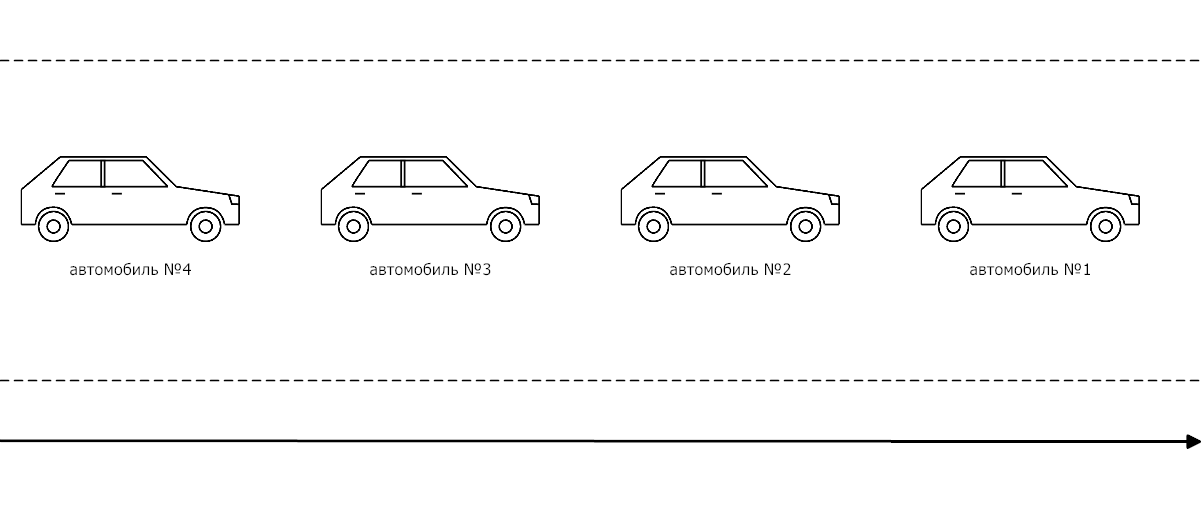
\includegraphics[keepaspectratio,width=160mm,height=70mm]{Images/car_following.png}
	\end{center}
	\caption{Автомобили, следующие друг за другом.}
	\label{car_following}
\end{figure}

Рассмотрим парадигму автомобиля, которая основана на очень простом правиле и уже довольно давно известна в литературе. Так как автомобили следуют друг за другом, преследователь всегда пытается максимизировать свою скорость с двумя ограничениями: ограничением ускорения и ограничением безопасности. Впервые данная парадигма была высказана ещё в 1975 \cite{GippsModel} и математически выглядит следующим образом:

\begin{equation} \label{following_paradigm}
v_f(t) = \min(v_f^d(t), v_f^s(t)),
\end{equation}
где $v_f(t)$ - скорость преследователя в момент времени $t$, $v_f^d(t)$ - максимальная возможная скорость с \textbf{ограничением ускорения} (demand speed), $v_f^s(t)$ - максимальная возможная скорость с \textbf{ограничением безопасности} (supply speed).

Под ограничение ускорения стоит понимать физические ограничения скорости и ускорения транспортного средства, а также условия комфорта, необходимые водителю. Это величина описывает траекторию транспортного средства, которое свободно разгоняется до максимальной желаемой скорости при отсутствии впереди идущих транспортных средств. Ограничение безопасности - это то, как траектория транспортного средства зависит от впереди идущего транспортного средства (лидера).

\section{Обзор, анализ и модификация существующих математических моделей}
\subsection{Модель свободного движения}

Для начала рассмотрим простую ситуацию, когда на дороге есть всего один автомобиль, для которого нет никаких ограничений, за исключением технических характеристик транспортного средства. В такой ситуации парадигму автомобиля \eqref{following_paradigm} можно записать следующим образом:

\begin{equation*}
v_f(t) = v_f^d(t),
\end{equation*}
то есть автомобиль разгонится до максимально желаемой скорости и будет продолжать с ней движение. Такое поведение будем называть свободным движением. 

Для описания свободного движения можно использовать хорошо известное обыкновенное дифференциальное уравнение вида: 
\begin{equation} \label{free_drive}
\begin{cases}
\begin{split}
\ddot{x}&(t) = \alpha\left( 1-\left( \dfrac{\dot{x}(t)}{v_{max}}\right)^\delta \right) \\
&x(0)=x_0, \quad \dot{x}(0)=v_{0}
\end{split}
\end{cases}.
\end{equation}
В уравнении \eqref{free_drive} за $x$ обозначено положение транспортного средства, а за $\dot{x}$ и $\ddot{x}$ скорость и ускорение соответственно.

Из уравнения \eqref{free_drive} видно, что свободное движение характеризуется максимально желаемой (допустимой) скоростью $v_{max}$, начальной скоростью $v_{0}$, начальным положением транспортного средства $x_0$, максимальным ускорением $\alpha$ и показателем степени $\delta$, определяющим, как ускорение уменьшается с ростом скорости.

В уравнении \eqref{free_drive} вынесем знаменатель за скобку и будем считать полученное выражение за коэффициент ускорения $a=\dfrac{\alpha}{v_{max}^\delta}$. Таким образом получаем следующую модель для свободного двигающегося автомобиля:

\begin{equation} \label{free_drive_with_initial_conditions}
\begin{cases}
\begin{split}
\ddot{x}&(t) = a\left( v_{max} - \dot{x}(t)\right)^\delta \\
&x(0)=x_0, \quad \dot{x}(0)=v_0
\end{split}
\end{cases}.
\end{equation}

Решения уравнения \eqref{free_drive_with_initial_conditions} имеет схожую динамику при различных значениях $\delta$. Это хорошо видно из рисунка \eqref{free_drive_with_delta}, на котором изображены графики\footnote{Все графики в данной работе выполнены с использованием системы компьютерной алгебры Wolfram Mathematica \cite{WolframMathematica}.} решения уравнения \eqref{free_drive_with_initial_conditions} при разных $\delta$.

\begin{figure}[h!]
	\begin{center}
		\begin{minipage}[h!]{0.48\linewidth}
			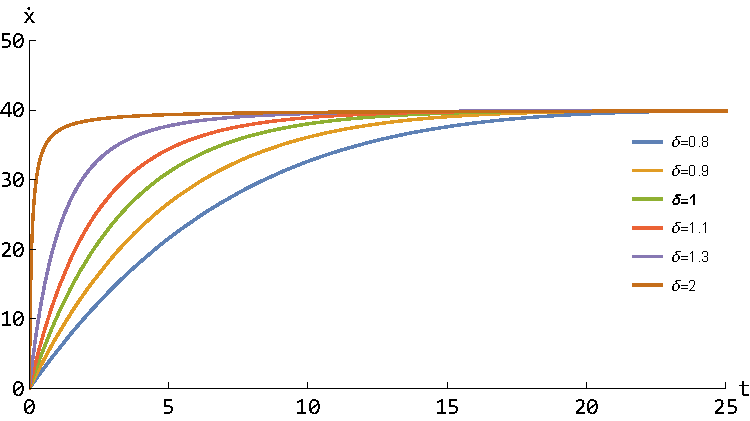
\includegraphics[width=1\linewidth,height=0.2\textheight]
			{Images/free_drive_speed_with_different_delta.pdf}
		\end{minipage}
		\caption{Графики изменения скорости при разных $\delta$ с параметрами: $a=0.15$, $v_{max}=40$, $x_0=0$, $v_0=0$.}
		\label{free_drive_with_delta}
	\end{center}
\end{figure}

Таким образом можно без потери общности рассматривать модель \eqref{free_drive_with_initial_conditions} при $\delta=1$, что соответствует линейному уменьшению ускорения с ростом скорости.

Система \eqref{free_drive_with_initial_conditions} при $\delta=1$ имеет решение в явном виде:
\begin{equation*}
x(t) =\dfrac{1}{a}\left(av_{max}t+v_{max}e^{-at}-v_{max}-v_0e^{-at}+v_0+ax_0\right) 
\end{equation*}
Из уравнения \eqref{free_drive_with_initial_conditions} видно, что при $v_0=v_{max}$ ускорения нет. Такое поведение согласуется с динамикой реального транспортного средства.

На рисунке \eqref{free_drive_without_stop} изображены графики скорости и расстояния для свободно двигающегося автомобиля.
\begin{figure}[h!]
	\begin{center}
		\begin{minipage}[h!]{0.48\linewidth}
			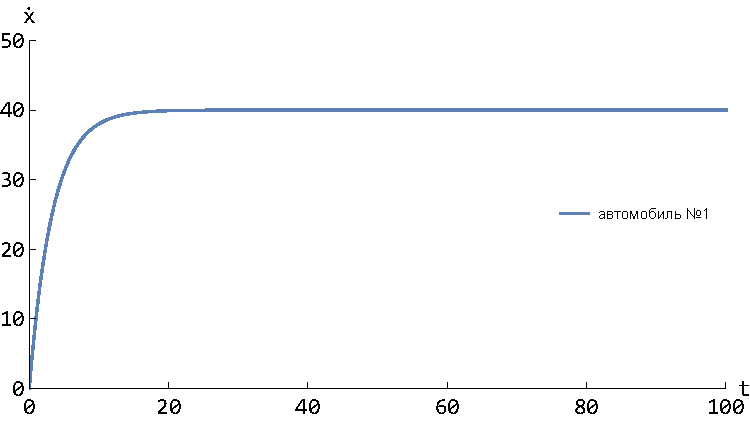
\includegraphics[width=1\linewidth,height=0.2\textheight]
			{Images/free_drive_speed.pdf}
		\end{minipage}
		\hfill 
		\begin{minipage}[h!]{0.48\linewidth}
			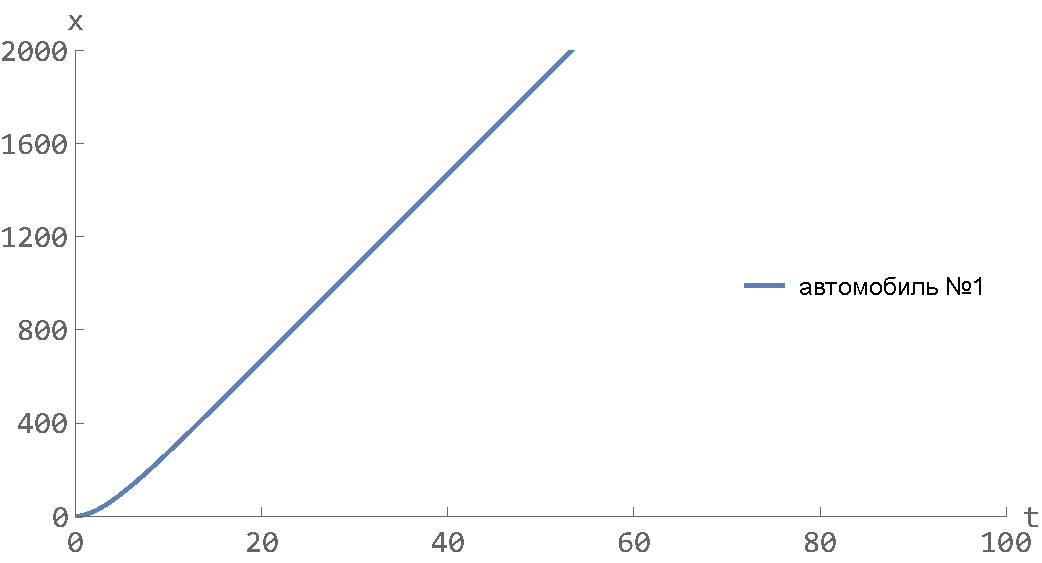
\includegraphics[width=1\linewidth,height=0.2\textheight]
			{Images/free_drive_distance.pdf}
		\end{minipage}
		\caption{Графики изменения скорости (слева) и расстояния (справа) для автомобиля при свободном движении без остановки с параметрами: $a=0.3$, $v_{max}=40$, $x_0=0$, $v_0=0$.}
		\label{free_drive_without_stop}
	\end{center}
\end{figure}

Из графиков видно, что автомобиль, разогнавшись до максимальной допустимой (желаемой) скорости, бесконечно двигается вперёд. Данная модель описывает момент старта автомобиля, его разгон и движение с постоянной скоростью. Под стартом автомобиля будем понимать момент начала разгона. В более жизненных ситуациях присутствуют процессы обратные разгону и старту - торможение и остановка.

Для описания остановки автомобиля рассмотрим дифференциальное уравнение, схожее с \eqref{free_drive_with_initial_conditions}: 
\begin{equation} \label{stop_drive_with_initial_conditions}
\begin{cases}
\begin{split}
\ddot{x}&(t) = q\left( v_{min} - \dot{x}(t)\right) \\
&x(0)=x_0, \quad \dot{x}(0)=v_0
\end{split}
\end{cases}.
\end{equation}
Из уравнения \eqref{stop_drive_with_initial_conditions} видно, что торможение характеризуется минимальной (желаемой) скоростью $v_{min}$, начальной скоростью $v_{0}$, начальным положением транспортного средства $x_0$ и коэффициентом торможения $q$. Под минимальной скоростью будем понимать такую скорость до которой водитель транспортного средства хочет снизить свою текущую скорость. Это не обязательно нулевая величина, в некоторых случаях водитель не хочет останавливаться полностью, а хочет лишь снизить скорость до какого-то значения.

Система \eqref{stop_drive_with_initial_conditions} имеет решение в явном виде, аналогичное системе \eqref{free_drive_with_initial_conditions}:
\begin{equation*}
x(t) = \dfrac{1}{q}\left(qv_{min}t+v_{min}e^{-qt}-v_{min}-v_0e^{-qt}+v_0+qx_0\right) 
\end{equation*}

Из уравнения \eqref{stop_drive_with_initial_conditions} видно, что при $v_0=v_{min}$ торможения нет. Данное поведение, аналогично случаю для ускорения, согласуется с динамикой реального транспортного средства.

Уравнения \eqref{free_drive_with_initial_conditions} и  \eqref{stop_drive_with_initial_conditions} описывают два разных вида движения. Для получения общей модели, описывающей оба этих вида движения, необходимо объединить их в одну. Предположим, что в нулевой момент времени происходит первая фаза движения - старт автомобиля и его разгон. Затем с некоторого момента времени $t_s$ (stop time) происходит вторая фаза движения - автомобиль начинает тормозить. Введём две релейные функции $R_{a}(t)$ и $R_{b}(t)$, вида:  

\begin{equation*} 
R_{a}(t)=
\begin{cases}
\begin{split}
&1, \quad&\text{если } t<t_{s} \\
&0, \quad&\text{если } t\geq t_{s}
\end{split}
\end{cases},
\qquad
R_{b}(t)=
\begin{cases}
\begin{split}
&0, \quad&\text{если } t<t_{s} \\
&1, \quad&\text{если } t\geq t_{s}
\end{split}
\end{cases}.
\end{equation*}
Релейная функция $R_{a}(t)$ ``включается'', когда автомобиль находится в фазе разгона (acceleration phase) и ``выключается'', когда автомобиль переходит в фазу торможения (braking phase). Функция $R_{b}(t)$ наоборот - ``выключается'' в фазе разгона и ``включается'' в фазе торможения. Функцию $R_{a}(t)$ можно выразить через $R_{b}(t)$ следующим образом $R_{a}(t) = (1-R_{b}(t))$. Обозначим $R_{a}(t)$ как $R(t)$ и получим релейную функцию, которая объединяет два вида движения.

\begin{equation} \label{relay_function}
R(t)=
\begin{cases}
\begin{split}
&1, \quad&\text{если } t<t_{s} \\
&0, \quad&\text{если } t\geq t_{s}
\end{split}
\end{cases}.
\end{equation}

С помощью полученной релейной функции \eqref{relay_function} объединим модели \eqref{free_drive_with_initial_conditions} и  \eqref{stop_drive_with_initial_conditions} и получим полную модель свободного движения:
\begin{equation} \label{free_drive_model}
\begin{cases}
\begin{split}
\ddot{x}(t) = &R(t) \left[ a\left(v_{max}-\dot{x}(t) \right)\right] + (1-R(t)) \left[ q\left( v_{min} - \dot{x}(t)\right) \right]  \\
&x(0)=x_0, \quad \dot{x}(0)=v_{0}
\end{split}
\end{cases}.
\end{equation}

Уравнения \eqref{free_drive_with_initial_conditions} и  \eqref{stop_drive_with_initial_conditions} различаются лишь коэффициентами и целевой скоростью $v_{target}$, под которой будем понимать скорость к которой стремится автомобиль во время движения. В случае ускорения это $v_{max}$, а в случае торможения $v_{min}$. С учётом данных предположений объединённую модель \eqref{free_drive_model} можно переписать в более компактном в виде:

\begin{equation} \label{free_drive_model_short}
\begin{cases}
\begin{split}
\ddot{x}(t) = &R_s(t) \left(v_{target}-\dot{x}(t) \right) \\
x(0)&=x_0, \quad \dot{x}(0)=v_{0}
\end{split}
\end{cases}.
\end{equation}
где $R_s(t)$ - релейная функция вида:
\begin{equation*}
R_s(t)=
\begin{cases}
\begin{split}
&a, \quad&\text{если } t<t_{s} \\
&q, \quad&\text{если } t\geq t_{s}
\end{split}
\end{cases}.
\end{equation*}

Модель \eqref{free_drive_model_short} эквивалентна \eqref{free_drive_model}, но менее информативна, так как в модели \eqref{free_drive_model} фазы разгона и торможения выделены в отдельные слагаемые.

На рисунке \eqref{free_drive_with_stop} изображены графики скорости и расстояния для свободно двигающегося автомобиля с остановкой по модели \eqref{free_drive_model}.

\begin{figure}[h!]
	\begin{center}
		\begin{minipage}[h!]{0.48\linewidth}
			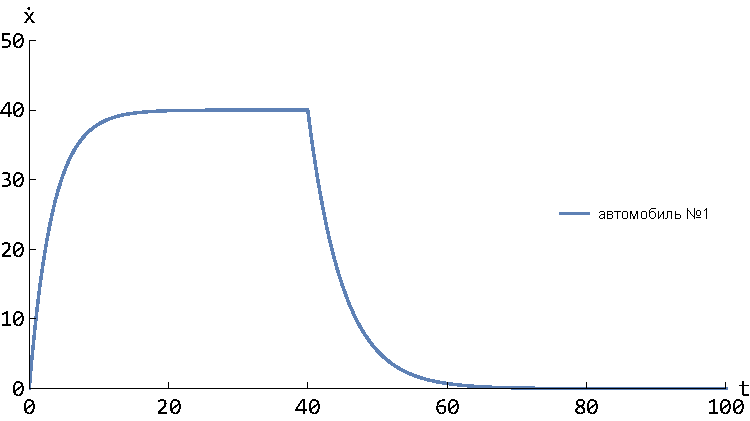
\includegraphics[width=1\linewidth,height=0.2\textheight]
			{Images/free_drive_speed_with_stop.pdf}
		\end{minipage}
		\hfill 
		\begin{minipage}[h!]{0.48\linewidth}
			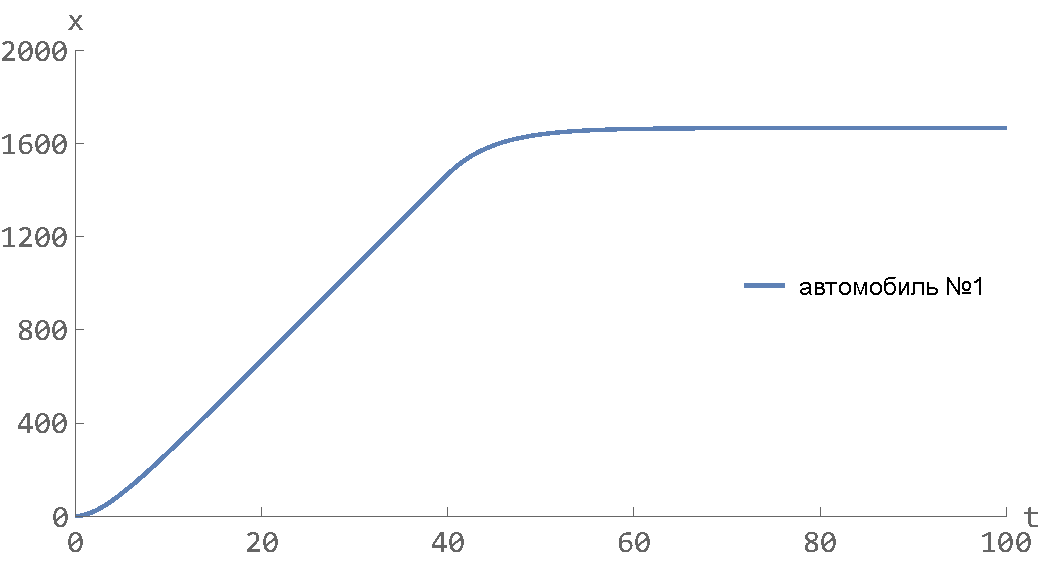
\includegraphics[width=1\linewidth,height=0.2\textheight]
			{Images/free_drive_distance_with_stop.pdf}
		\end{minipage}
		\caption{Графики изменения скорости (слева) и расстояния (справа) для автомобиля при свободном движении без остановки с параметрами: $a=0.3$, $q=0.2$, $v_{max}=40$, $v_{min}=0$, $t_s=40$, $x_0=0$, $v_0=0$.}
		\label{free_drive_with_stop}
	\end{center}
\end{figure}

Из графиков видно, что автомобиль, разогнавшись до максимальной допустимой (желаемой) скорости, двигается с ней до наступления времени торможения. Затем автомобиль начинает тормозить до минимальной желаемой скорости и продолжает с ней движение или же, если минимальная скорость равна нулю ($v_{min}=0$), как на графиках \eqref{free_drive_with_stop}, останавливается.
 
Таким образом была получена модель \eqref{free_drive_model}, которая описывает все значимые фазы движения одного автомобиля, а именно разгон, само движение и торможение. Даная модель не учитывает внешних факторов, которые оказывают влияние на движение автомобиля, она зависит лишь от технических характеристик транспортного средства и от самого водителя. Эта модель подходит для описания динамики первого автомобиля в потоке. На остальные автомобили большое влияние оказывают впереди идущие транспортные средства, поэтому они вынуждены двигаться учитывая движение лидера.

\subsection{``Простая'' модель следования за лидером}

Рассмотрим несколько автомобилей и занумеруем их индексом $n \in \mathbb{N}$ в соответствии с их порядковым номером на дороге. Предполагается, что ускорение $n$-ого автомобиля определяется состоянием соседних автомобилей, а именно наибольшее влияние оказывает непосредственно впереди идущий автомобиль (лидер).

Первая модель, основанная на принципе следования за лидером была разработана в 50-х годах прошлого века и предполагала, что каждый водитель адаптирует свою скорость к скорости лидирующего автомобиля:

\begin{equation} \label{follow_the_leader_first_model}
\ddot{x}_n(t) = \dfrac{1}{\gamma} (\dot{x}_{n-1}(t) - \dot{x}_{n}(t)), 
\end{equation}
где $\gamma$ - время адаптации водителя.

Данное уравнение было получено в работе Пайпса (Pipes) \cite{FirstFollowTheLeaderModel}. Модель, построенная на основе данного уравнения, является простой и плохо описывает свойства реального транспортного потока \cite{Shvetsov}.

В работе \cite{RefineFirstFollowTheLeaderModel} была предложена модификация уравнения \eqref{follow_the_leader_first_model}. В левую часть уравнения была введена задержка аргумента по времени $\tau$, которая отражает время реакции водителей на изменение скорости лидирующего автомобиля. 

\begin{equation*}
\ddot{x}_n(t+\tau) = \dfrac{1}{\gamma} (\dot{x}_{n-1}(t) - \dot{x}_{n}(t)).
\end{equation*}
Произведя замену времени получим следующие уравнение:
\begin{equation} \label{follow_the_leader_with_two_delay}
\ddot{x}_n(t) = \dfrac{1}{\gamma} (\dot{x}_{n-1}(t-\tau) - \dot{x}_{n}(t-\tau)).
\end{equation}

Уравнение \eqref{follow_the_leader_with_two_delay} содержит запаздывание в двух слагаемых в правой части, то есть ускорение автомобиля зависит от разности скоростей, которые были у текущего и впереди идущего автомобилей $\tau$ времени назад.

Упростим уравнение \eqref{follow_the_leader_with_two_delay}, оставив в правой части запаздывание только у первого слагаемого, таким образом ускорение автомобиля будет зависеть от его текущей скорости и скорости впереди идущего автомобиля $\tau$ времени назад. Множитель $\dfrac{1}{\gamma}$ будем интерпретировать как коэффициент мощности $d$, характеризующий мощность двигателя автомобиля. С учётом проведённых модификаций уравнение примет вид:

\begin{equation} \label{follow_the_leader_with_delay}
\ddot{x}_n(t) = d_{n} (\dot{x}_{n-1}(t-\tau) - \dot{x}_{n}(t)).
\end{equation}

Без потери общности будем считать, что все автомобили имеют одинаковые технические характеристики $d_n = d$, а все водители одинаково оценивают дорожную ситуацию и реагируют на её изменения с одинаковой скоростью.

Уравнение \eqref{follow_the_leader_with_delay} можно проинтегрировать и рассматривать модель, которая описывает скорость и зависит от положения самого автомобиля и положения лидера. Данный подход подробно описан в \cite{Course}, в данной работе будем рассматривать уравнение в исходном виде. 

Уравнение \eqref{follow_the_leader_with_delay} не описывает движение первого автомобиля и для описания динамики первого автомобиля дополним уравнение \eqref{follow_the_leader_with_delay} ранее полученным уравнением свободного движения \eqref{free_drive_model}, остальные автомобили будут двигаться согласно разностному уравнению \eqref{follow_the_leader_with_delay}. Будем считать, что в начальный момент времени все автомобили находятся на равном  расстоянии $\lambda$ друг от друга.

\begin{equation} \label{follow_the_leader_full_model}
\begin{cases}
\begin{split}
\ddot{x}_1(t)& = R(t) \left[ a\left(v_{max}-\dot{x}_1(t) \right)\right] + (1-R(t)) \left[ q\left( v_{min} - \dot{x}_1(t)\right) \right] \\
&x_{1}(0)=x_0, \quad \dot{x}_{1}(0)=v_{0}\\
\ddot{x}_{n}(t)& = d(\dot{x}_{n-1}(t-\tau)-\dot{x}_{n}(t)) \\
&x_n(t)=x_0-(n-1)\lambda, \quad \dot{x}_n(t)=v_{n}, \quad \text{при } t \in [-\tau,0] \text{ и } n\geq2
\end{split}
\end{cases},
\end{equation}

На рисунке \eqref{follow_the_leader} изображены графики скорости и расстояния для нескольких автомобилей, движущихся друг за другом.

\begin{figure}[h!]
	\begin{center}
		\begin{minipage}[h!]{0.48\linewidth}
			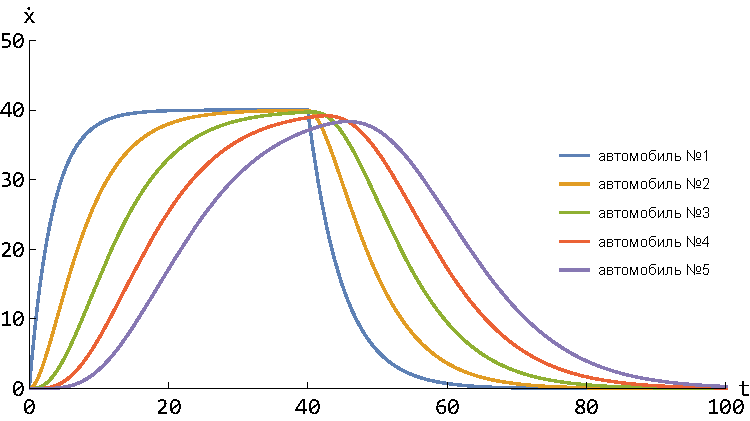
\includegraphics[width=1\linewidth,height=0.2\textheight]
			{Images/simple_model_speed.pdf}
		\end{minipage}
		\hfill 
		\begin{minipage}[h!]{0.48\linewidth}
			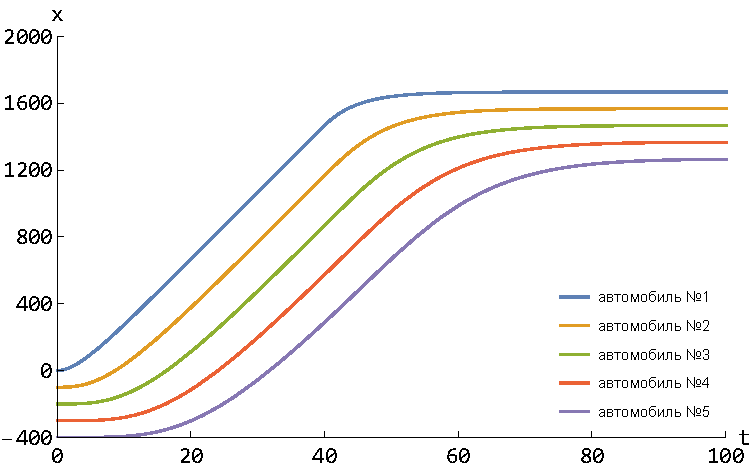
\includegraphics[width=1\linewidth,height=0.2\textheight]
			{Images/simple_model_distance.pdf}
		\end{minipage}
		\caption{Графики изменения скорости (слева) и расстояния (справа) для транспортного потока с остановкой с параметрами: $\tau=1$, $a=0.3$, $q=0.2$, $v_{max}=40$, $v_{min}=0$, $\lambda=100$, $d=0.2$, $t_s=40$, $x_0=0$, $v_n=0$, $v_0=0$.}
		\label{follow_the_leader}
	\end{center}
\end{figure}

Из графиков видно, что автомобили, разгоняются до максимальной желаемой скорости и двигаются до момента времени $t_s$, начиная с которого, первый автомобиль тормозит и останавливается. Остальные автомобили, повторяя динамику первого автомобиля, так же останавливаются. Все движение происходит с сохранением безопасной дистанции между автомобилями, что соответствует реальному транспортному потоку, так как сокращение безопасного расстояния подразумевает появление аварийной ситуации.

Результаты исследования модели \eqref{follow_the_leader_full_model} совпадают с  результатами исследований моделей \eqref{follow_the_leader_with_two_delay} и проинтегрированной \eqref{follow_the_leader_full_model} из работ \cite{RefineFirstFollowTheLeaderModel} и \cite{Course} соответственно. С помощью регулировки коэффициентов в моделях можно добиться полной идентичности решений. Данные модели не учитывают расстояния между транспортными средствами, имеют сравнительно простую динамику, и могут быть в равной мере использованы для моделирования движения транспортных потоков. 

\subsection{Модель следования за лидером ``Дженерал моторс''}

Группа инженеров из компании ``Дженерал моторс'' (General Motors) в своей работе \cite{GazisModel} предложила дополнительную модификацию для уравнения  \eqref{follow_the_leader_with_two_delay}. Основной этой модификации является идея рассмотреть вместо постоянного коэффициента $\dfrac{1}{\gamma}$ динамическую величину $S(t)$, которую можно интерпретировать как коэффициент чувствительности. 

Коэффициент чувствительности $S(t)$ характеризует скорость реакции водителя к изменению скорости лидера и зависит от скорости и текущей дистанции до лидера. Чувствительность возрастает при уменьшении дистанции до лидера, таким образом коэффициент $S(t)$ можно представить в виде:

\begin{equation} \label{gazis_coefficient}
S(t) = \dfrac{\eta_{l,m}\dot{x}_n^{m_1}(t)}{(x_{n-1}(t-\tau)-x_n(t-\tau))^{m_2}},
\end{equation}
где $\eta$ - константа, характеризующая движение, а $m_1$ и $m_2$ - эмпирически подбираемые константы, характеризующие движение. Данный коэффициент был получен в работе Газиса, Хермана и Ротери (Gazis-Herman-Rothery, GHR)  \cite{GazisModel}, и модель, полученная с учётом сделанных преобразований выглядит следующим образом:   
\begin{equation} \label{gazis_model}
\ddot{x}_n(t) = \dfrac{\eta_{l,m}\dot{x}_n^{m_1}(t)}{(x_{n-1}(t-\tau)-x_n(t-\tau))^{m_2}} (\dot{x}_{n-1}(t-\tau) - \dot{x}_{n}(t-\tau)).
\end{equation}

Изучение модели, полученной Газисом-Херманом-Ротери, в исходном виде описано в работах \cite{StudyingGazisModel_1},  \cite{StudyingGazisModel_2} и  \cite{StudyingGazisModel_3}. При значениях параметров $m_1 \approx 0.8$, $m_2 \approx 2.8$ \cite{StudyingGazisModel_1} или $m_1 = 0.953$, $m_2 = 3.05$ \cite{StudyingGazisModel_2}, \cite{StudyingGazisModel_3} получаются результаты наиболее схожие с реальными данными.

Аналогично ``простой'' модели, данная модель \eqref{gazis_model} плохо описывать движение первого автомобиля, поэтому дополним его уравнением \eqref{free_drive_model} и рассмотрим полученную модель движения транспортного потока:

\begin{equation} \label{full_gazis_model}
\begin{cases}
\begin{split}
\ddot{x}_1(t)& = R(t) \left[ a\left(v_{max}-\dot{x}_1(t) \right)\right] + (1-R(t)) \left[ q\left( v_{min} - \dot{x}_1(t)\right) \right] \\
&x_{1}(0)=x_0, \quad \dot{x}_{1}(0)=v_{0}\\
\ddot{x}_n(t)& = \dfrac{\eta_{l,m}\dot{x}_n^{m_1}(t)}{(x_{n-1}(t-\tau)-x_n(t-\tau))^{m_2}} (\dot{x}_{n-1}(t-\tau) - \dot{x}_{n}(t-\tau)) \\
&x_n(t)=x_0-(n-1)\lambda, \quad \dot{x}_n(t)=v_{n}, \quad \text{при } t \in [-\tau,0] \text{ и } n\geq2
\end{split}
\end{cases}.
\end{equation}

Полученные модели \eqref{gazis_model} и \eqref{full_gazis_model} очень сильно зависят от эмпирически подбираемых констант $m_1$ и $m_2$. При неудачном выборе данных констант решения не согласуются с реальными данными. На рисунках \ref{gazis_model_good} и \ref{gazis_model_bad} изображены графики решений для ``удачного'' и ``неудачного'' выбора параметров. 
\begin{figure}[h!]
	\begin{center}
		\begin{minipage}[h!]{0.48\linewidth}
			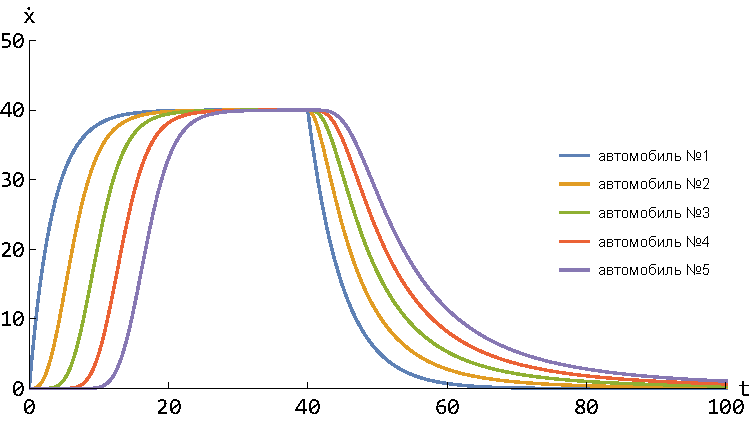
\includegraphics[width=1\linewidth,height=0.2\textheight]
			{Images/gazis_model_good_speed.pdf}
		\end{minipage}
		\hfill 
		\begin{minipage}[h!]{0.48\linewidth}
			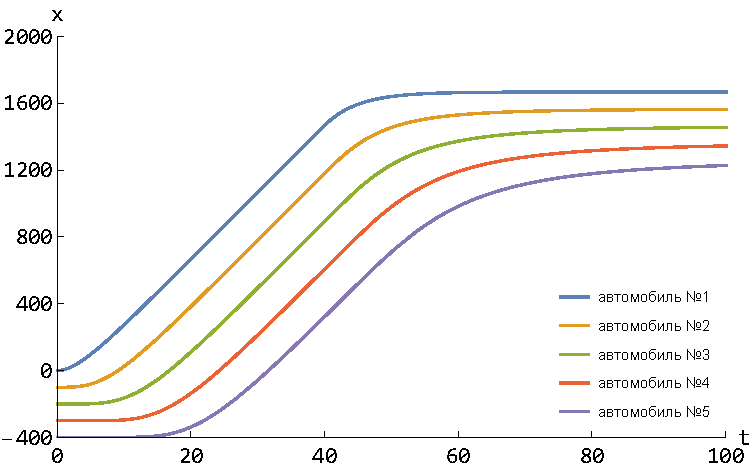
\includegraphics[width=1\linewidth,height=0.2\textheight]
			{Images/gazis_model_good_distance.pdf}
		\end{minipage}
		\caption{Графики изменения скорости (слева) и расстояния (справа) для модели Газиса-Хермана-Ротери с ``удачным'' выбором параметров: $\tau=1$, $a=0.3$, $q=0.2$, $v_{max}=40$, $v_{min}=0$, $\lambda=100$, $t_s=40$, $x_0=0$, $v_0=0$, $\eta=0.4$, $\boldsymbol{m_1=0.4}$, $\boldsymbol{m_2=0.3}$}
		\label{gazis_model_good}
	\end{center}
\end{figure}

\begin{figure}[h!]
	\begin{center}
		\begin{minipage}[h!]{0.48\linewidth}
			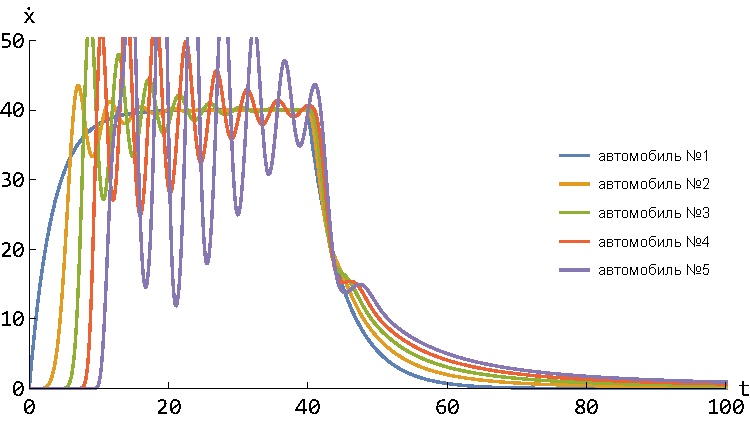
\includegraphics[width=1\linewidth,height=0.2\textheight]
			{Images/gazis_model_bad_speed.pdf}
		\end{minipage}
		\hfill 
		\begin{minipage}[h!]{0.48\linewidth}
			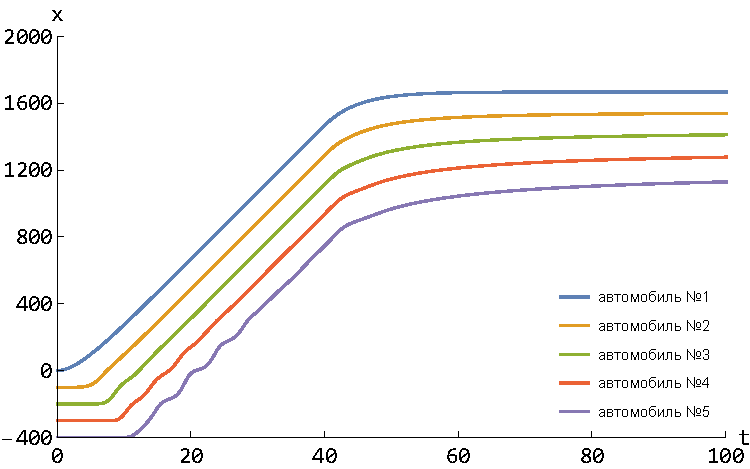
\includegraphics[width=1\linewidth,height=0.2\textheight]
			{Images/gazis_model_bad_distance.pdf}
		\end{minipage}
		\caption{Графики изменения скорости (слева) и расстояния (справа) для модели Газиса-Хермана-Ротери с ``неудачным'' выбором параметров: $\tau=1$, $a=0.3$, $q=0.2$, $v_{max}=40$, $v_{min}=0$, $\lambda=100$, $t_s=40$, $x_0=0$, $v_0=0$, $v_n=0$, $v_n=0$, $\eta=0.4$, $\boldsymbol{m_1=0.7}$, $\boldsymbol{m_2=0.3}$}
		\label{gazis_model_bad}
	\end{center}
\end{figure}

Графики на рисунке \ref{gazis_model_good} демонстрируют хорошую ситуацию, когда решения согласуются с реальным поведением транспортных средств на дороге. Графики на рисунке \ref{gazis_model_bad} показывают плохую ситуацию. Скорость некоторых автомобилей с некоторого момента времени начинает сильно колебаться с большой амплитудой и не только превышает допустимую скорость, но и в некоторых случаях падает почти до нуля. Такое поведение невозможно в реальной жизни.

Из результатов исследования можно сделать вывод, что ни данная модель в исходном виде \eqref{gazis_model} ни данная модель, дополненная уравнением движения первого автомобиля \eqref{full_gazis_model}, не подходят для моделирования движения автомобилей. Большая зависимость от правильного выбора параметров $m_1$ и $m_2$ и несвязанность этих параметров с каким-то физическими величинами очень усложняет моделирование и не гарантирует получение правильной динамики движения транспортных потоков. 

\subsection{Модель ``разумного водителя''}
В настоящее время наиболее современной и популярной моделью движения транспортных потоков является модель ``разумного водителя'' (Intelligent Driver Model, IDM), разработанная Трайбером с соавторами \cite{TreiberModel_1}, \cite{TreiberModel_2} в конце прошлого начале нынешнего века. 

В модели ``разумного водителя'' ускорение автомобиля зависит от текущей скорости самого автомобиля, от скорости впереди идущего автомобиля и расстояния между ними. Математически это можно записать в следующем виде:
\begin{equation*}
\ddot{x}_n(t)=f(t, \dot{x}_n,\dot{x}_{n-1}, x_{n-1}-x_n).
\end{equation*} 

В модели ``разумного водителя'' движение автомобиля состоит из двух фаз. Первая фаза - это фаза разгона, в которой автомобиль пытается разогнаться до максимальной допустимой скорости. Вторая фаза - фаза торможения, в которой автомобиль замедляется, что бы держаться на безопасном расстоянии от впереди идущей машины.
\begin{equation} \label{treiber_model}
\ddot{x}_n(t)= \alpha\left( 1-\left( \dfrac{\dot{x}_n(t)}{v_{max}}\right)^\delta \right) - \alpha\left( \dfrac{s^*_n(\dot{x}_n(t),\Delta \dot{x}_n(t))}{s_n}\right)^2,
\end{equation}
где $s_n$ - фактическое расстояние между автомобилями, а $s^*_n$ - желаемое.

Фактическое расстояние $s_n$ определяется разницей между положениями двух соседних автомобилей $s_n=x_{n-1}(t)-x_n(t)$. Желаемое расстояние  $s^*_n$ определяется формулой:
\begin{equation*}
s^*_n = \sigma_0+\sigma_1\sqrt{\dfrac{ \dot{x}_n(t)}{v_{max}}} +T \dot{x}_n(t)+ \dfrac{ \dot{x}_n(t)\Delta \dot{x}_n(t) }{2\sqrt{ab}},
\end{equation*}
где $\Delta \dot{x}_n(t) = \dot{x}_n(t)- \dot{x}_{n-1}(t)$ - разница скоростей автомобилей, $\sigma_0$ - расстояние между автомобилями, $\sigma_1$ - коэффициент регулировки скорости в заторе, $T$ - безопасный временной интервал, $b$ - коэффициент ``комфортного'' (не экстренного) торможения.

Можно заметить, что в модели \eqref{treiber_model} первое слагаемое - это модель свободного движения в исходном виде \eqref{free_drive}, а второе - это усовершенствованный коэффициент чувствительности \eqref{gazis_coefficient} из модели Газиса-Хермана-Ротери. Таким образом, можно сделать вывод, что в модели ``разумного водителя'' объединяются лучшие идеи предыдущих моделей.

Аналогично модели свободного движения рассмотрим модель ``разумного водителя'' \eqref{treiber_model} при линейном уменьшении ускорения с ростом скорости $\delta=1$.

\begin{equation} \label{full_treiber_model}
\ddot{x}_n(t)= \alpha\bigg(\dfrac{v_{max}-\dot{x}_n(t)}{v_{max}} \bigg) - \alpha\bigg( \dfrac{\sigma_0+\sigma_1\sqrt{\frac{ \dot{x}_n(t)}{v_{max}}} +T \dot{x}_n(t)+ \frac{ \dot{x}_n(t)\Delta \dot{x}_n(t) }{2\sqrt{ab}}}{x_{n-1}(t)-x_n(t)}\bigg)^2.
\end{equation}

Аналогично двум предыдущим случая данная модель \eqref{full_treiber_model} плохо описывает динамику первого автомобиля, поэтому дополним её уравнением для первого автомобиля \eqref{free_drive_model} и рассмотрим полученную модель движения транспортного потока:
\begin{equation} \label{full_treiber_model_with_first_car} 
\begin{cases}
\begin{split}
\ddot{x}_1(t)& = R(t) \left[ a\left(v_{max}-\dot{x}_1(t) \right)\right] + (1-R(t)) \left[ q\left( v_{min} - \dot{x}_1(t)\right) \right] \\
&x_{1}(0)=x_0, \quad \dot{x}_{1}(0)=v_{0}\\
\ddot{x}_n(t)& = \alpha\bigg(\dfrac{v_{max}-\dot{x}_n(t)}{v_{max}} \bigg) - \alpha\bigg( \dfrac{\sigma_0+\sigma_1\sqrt{\frac{ \dot{x}_n(t)}{v_{max}}} +T \dot{x}_n(t)+ \frac{ \dot{x}_n(t)\left[ \dot{x}_n(t)-\dot{x}_{n-1}(t)\right]  }{2\sqrt{ab}}}{x_{n-1}(t)-x_n(t)}\bigg)^2 \\
&x_n(t)=x_0-(n-1)\lambda, \quad \dot{x}_n(t)=v_{n}, \quad \text{при } t \in [-\tau,0] \text{ и } n\geq2
\end{split}
\end{cases}.
\end{equation}

На рисунке \eqref{treiber_model_img} изображены графики скорости и расстояния для нескольких автомобилей, движущихся друг за другом, согласно модели \eqref{full_treiber_model_with_first_car}.

\begin{figure}[h!]
	\begin{center}
		\begin{minipage}[h!]{0.48\linewidth}
			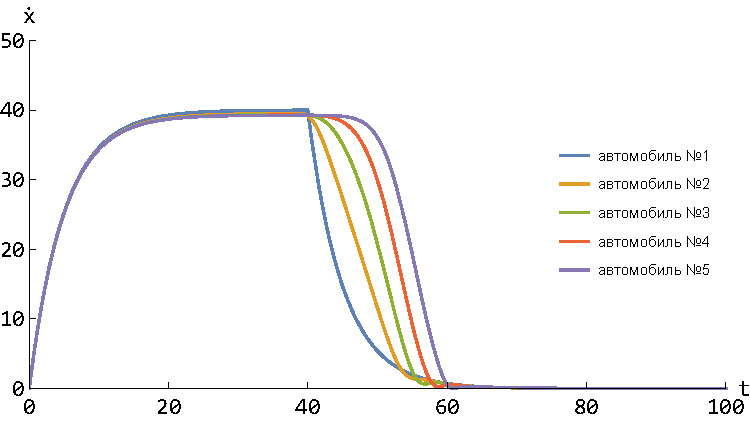
\includegraphics[width=1\linewidth,height=0.2\textheight]
			{Images/treiber_model_speed.pdf}
		\end{minipage}
		\hfill 
		\begin{minipage}[h!]{0.48\linewidth}
			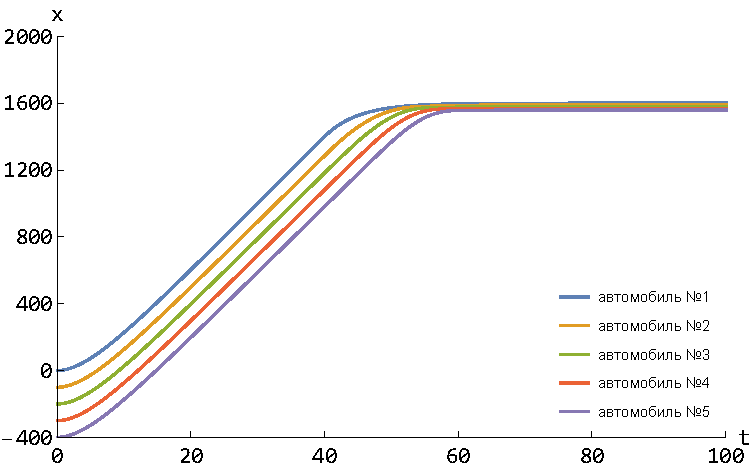
\includegraphics[width=1\linewidth,height=0.2\textheight]
			{Images/treiber_model_distance.pdf}
		\end{minipage}
		\caption{Графики изменения скорости (слева) и расстояния (справа) для модели Трайбера с параметрами: $a=0.2$, $\alpha=8$, $q=0.2$, $v_{max}=40$, $v_{min}=0$, $\lambda=100$, $t_s=40$, $x_0=0$, $v_0=0$, $v_n=0$, $\sigma_0=10$,$\sigma_1=5$, $T=0.1$, $b=2$ }
		\label{treiber_model_img}
	\end{center}
\end{figure}

На графиках \eqref{treiber_model_img} видна не совсем корректная динамика. Так из графика скорости видно, что автомобили не достигают максимальной возможной скорости, так как скорости автомобилей отделены друг от друга на некоторую величину. Также на из графика скорости видно, что при остановке скорость автомобиля начинает колебаться, из-за чего между автомобилями не остаётся расстояния. Такое поведение не соответствует динамике движения реального транспортного потока. 

Таким образом модель ``разумного водителя'' в исходном виде не подходит для моделирования динамики транспортных потоков. Некорректная динамика и большое количества параметров делают модель непригодной для использования.

Улучшить модель ``разумного водителя'' можно путём сокращения параметров. Так, например, параметры $\sigma_1$ (коэффициент регулировки скорости в заторе) и $T$ (безопасный временной интервал) имеют неясную содержательную интерпретацию и могут быть занулены. Данная модификация упрощает модель, но не меняет её динамику, тем самым сохраняя несоответствие реальным данным.

\section{Построение новой математической модели}
Рассмотренные ранее модели обладают рядом недостатков и могут быть лишь частично использованы для моделирования транспортных потоков. 

Используя опыт и некоторые идеи ранее рассмотренных модель, построим новую модель, которая будет описывать движение $n \in \mathbb{N}$ автомобилей. Аналогично предыдущим моделям обозначим за $x$ положение транспортного средства, а за $\dot{x}$ и $\ddot{x}$ их скорость и ускорение соответственно. 

Все движение автомобиля разделим на две фазы: ускорение и торможение, причём в конкретный момент времени автомобиль либо разгоняется, либо тормозит. Для этого введём релейную функцию вида:

\begin{equation*}
R(\Delta x_{n}(t,\tau))=
\begin{cases}
\begin{split}
&1,\quad &\text{если }\Delta x_{n}(t,\tau) >S \\
&0,\quad &\text{если }\Delta x_{n}(t,\tau) \leq S
\end{split}
\end{cases},
\end{equation*}
где $\tau$ - время реакции водителя, $\Delta x_{n}(t,\tau)=x_{n-1}(t-\tau)-x_n(t)$ - расстояние между соседними автомобилями, а $S$ - тормозной путь. \textbf{Тормозной путь} - расстояние, которое проходит транспортное средство с момента срабатывания тормозной системы до полной остановки \cite{PDD}. Для расчёта тормозного пути воспользуемся хорошо известной формулой \cite{Physics}.
\begin{equation*} 
S=\dfrac{v^2}{2\mu g},
\end{equation*}
где $v$ - текущая скорость транспортного средства, $\mu$ - коэффициент трения, $g$ - ускорение свободного падения. Из определения тормозного пути следует, что автомобиль остановится вплотную к впереди идущему автомобилю, в случае его моментальной остановки. Для того чтобы разделить автомобили, к тормозному пути прибавим дополнительную единицу расстояния $S+1$. Объединив эти формулы получаем реле, которое будет переключать фазы движения автомобиля.
\begin{equation}\label{rele}
R(\Delta x_{n}(t,\tau))=
\begin{cases}
\begin{split}
&1,\quad &\text{если }\Delta x_{n}(t,\tau) > \dfrac{\dot{x}_n^2(t)}{2\mu g}+1 \\
&0,\quad &\text{если }\Delta x_{n}(t,\tau) \leq \dfrac{\dot{x}_n^2(t)}{2\mu g}+1
\end{split}
\end{cases}.
\end{equation}

Первая фаза движения - это разгон. Для описания разгона используем принцип, при котором преследующий автомобиль подстраивает свою скоростью относительно впереди идущего:

\begin{equation*}
\ddot{x}_n(t)= \bigg[ a(\dot{x}_{n-1}(t-\tau)-\dot{x}_n(t))\bigg],
\end{equation*}
где $a$ - коэффициент ускорения.

Вторая фаза движения - это торможение. Торможение автомобиля зависит от разности между расстояний и скоростей самого автомобиля и впереди идущего, а так же от безопасной дистанции между ними. Математически это можно записать следующим образом: 

\begin{equation*}
\ddot{x}_n(t)= \left[  q\left(  \dfrac{\dot{x}_n^2(t)\left[  \dot{x}_{n-1}(t-\tau) - \dot{x}_n(t) \right]}{(x_{n-1}(t-\tau)-x_n(t)-l)^2}\right) \right],
\end{equation*}
где $l$ - безопасное расстояние между автомобилями, a $q$ - коэффициент торможения.

Таким образом объединяя обе фазы получаем математическую модель движения транспортных потоков:
\begin{equation} \label{my_model} 
\begin{split}
\ddot{x}_n(t)= &R(\Delta x_n(t,\tau))\bigg[ a(\dot{x}_{n-1}(t-\tau)-\dot{x}_n(t))\bigg]  +\\+& (1-R(\Delta x_n(t,\tau)))\left[  q\left(  \dfrac{\dot{x}_n^2(t)\left[  \dot{x}_{n-1}(t-\tau) - \dot{x}_n(t) \right]}{(x_{n-1}(t-\tau)-x_n(t)-l)^2}\right) \right] 
\end{split}.
\end{equation}

Данная разностная модель описывает все автомобили потока. Для описания первого автомобиля модель необходимо дополнить начальными данными. Таким образом для первого автомобиля (при $n=1$) доопределим значения $x_{0}$ и $\dot{x}_{0}$.За $x_{0}$ будем считать расстояние, которое должен проехать автомобиль, например это может быть расстояние до светофора или иного препятствия $x_{0}=L$. За $\dot{x}_{0}$ в первом слагаемом будем считать максимальную желаемую скорость $\dot{x}_{0}=v_{max}$, а во втором минимальную желаемую скорость, то есть скорость до которой нужно оттормозиться $\dot{x}_{0}=v_{min}$.

Будем считать, что в начальный момент времени все автомобили находятся на расстоянии $\lambda$ от первого автомобиля, который находится в положении $\lambda_0$. Причём начальное положение автомобилей строго больше, чем расстояние во время движения, то есть $\lambda > l$.

Добавив начальные условия к модели \eqref{my_model} получаем полную математическую модель:

\begin{equation} \label{new_model} 
\begin{cases}
\begin{split}
\ddot{x}_n(t)= &R(\Delta x_n(t,\tau))\bigg[ a(\dot{x}_{n-1}(t-\tau)-\dot{x}_n(t))\bigg]  +\\+& (1-R(\Delta x_n(t,\tau)))\left[  q\left(  \dfrac{\dot{x}_n^2(t)\left[  \dot{x}_{n-1}(t-\tau) - \dot{x}_n(t) \right]}{(x_{n-1}(t-\tau)-x_n(t)-l)^2}\right) \right] \\
 \quad x_n(t)&=\lambda_0-(n-1)\lambda, \quad \dot{x}_n(t)=v_{n}, \quad \text{при } t \in [-\tau,0] \text{ и } n\geq2
\end{split}
\end{cases}.
\end{equation}

На рисунке \ref{new_model_picture} изображены графики скорости и расстояния для нескольких автомобилей, двигающихся друг за другом, согласно модели \eqref{new_model}.

\begin{figure}[h!]
	\begin{center}
		\begin{minipage}[h!]{0.48\linewidth}
			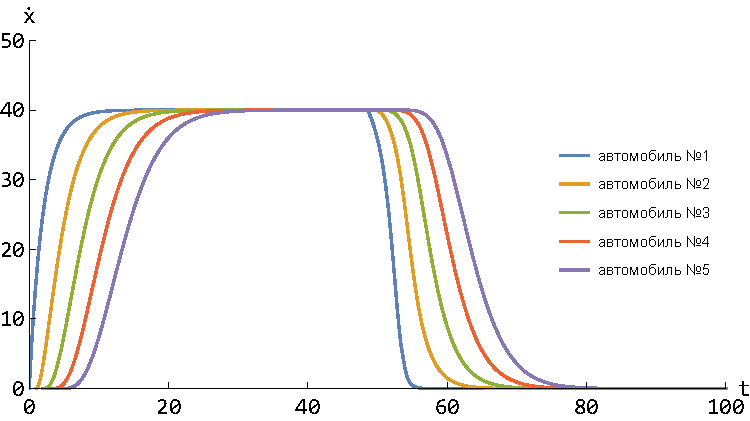
\includegraphics[width=1\linewidth,height=0.2\textheight]
			{Images/new_model_speed.pdf}
		\end{minipage}
		\hfill 
		\begin{minipage}[h!]{0.48\linewidth}
			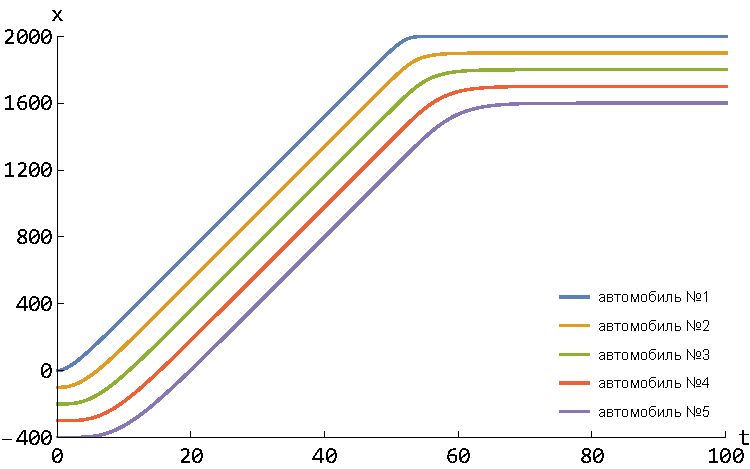
\includegraphics[width=1\linewidth,height=0.2\textheight]
			{Images/new_model_distanse.pdf}
		\end{minipage}
		\caption{Графики изменения скорости (слева) и расстояния (справа) для новой модели с параметрами: $a=0.5$, $q=0.6$, $v_{max}=40$, $v_{min}=0$, $\lambda=100$, $l=90$, $L=2000$, $x_0=0$, $v_n=0$, $g=9.8$, $\mu=0.6$ }
		\label{new_model_picture}
	\end{center}
\end{figure}

На графиках видна динамика, которая согласуется с динамикой реального транспортного потока. Автомобили разгоняются до максимальной допустимой скорости, а затем останавливаются на безопасном расстоянии. 

Модель \eqref{my_model} согласуется с реальной наблюдаемой ситуацией только на небольшом расстоянии между транспортными средствами, так как на большом расстоянии автомобилю нет смысла подстраивать свою скорость под скорость впереди идущей машины. Введём понятие \textbf{``расстояние влияния''}, под которым будем понимать такое расстояние, начиная с которого впереди идущий автомобиль оказывает влияние на позади идущий. В качестве ``расстояние влияния'' можно взять двойной тормозной путь $2S$. Таким образом, если расстояние между автомобилями большем, чем  $2S$, то преследующий автомобиль старается максимизировать свою скорость, если меньше, чем  $2S$, то преследующий автомобиль подстраивает свою скорость относительно впереди идущего. Математически это можно записать в виде релейной функции:

\begin{equation*}
F(\Delta x_{n}(t,\tau))=
\begin{cases}
\begin{split}
&v_{max},\quad &\text{если }\Delta x_{n-1,n}(t,\tau) > 2\dfrac{\dot{x}_n^2(t)}{2\mu g} \\
&\dot{x}_{n-1}(t-\tau),\quad &\text{если }\Delta x_{n-1,n}(t,\tau) \leq 2\dfrac{\dot{x}_n^2(t)}{2\mu g}
\end{split}
\end{cases}.
\end{equation*}

В реальной жизни максимальная комфортная скорость может быть своя у каждого автомобиля $v_{n,max}$, поэтому в некоторых случаях может возникнуть ситуация, когда впереди идущее транспортное средство движется со скоростью больше, чем максимальная комфортная скорость позади идущего. Для решения такой проблемы применим к первому слагаемому можно применить функцию Хевисайда \cite{Heaviside_function}, вида:
\begin{equation*}
\theta(\dot{x}_n(t))=
\begin{cases}
\begin{split}
&v_{n,max},\quad &\text{если }\dot{x}_n(t)>v_{n,max} \\
&\dot{x}_n(t),\quad &\text{если }\dot{x}_n(t)>v_{n,max}
\end{split}
\end{cases}.
\end{equation*}

Полученная математическая модель транспортных потоков согласуется с динамикой реального транспортного потока, и описывает все автомобили, включая первый. Применим новую модель для описания реальной дорожной ситуации.

\section{Практическое применение новой математической модели} 

\subsection{Подбор параметров} 

Прежде чем применять новую математическую модель \eqref{new_model} для моделирования реального транспортного потока необходимо ввести систему единиц измерения для параметров, использующихся в модели.

Размерности для величин: времени, расстояния и скорости возьмём из международной системы единиц (СИ). Таким образом время будем измерять в секундах (с), расстояние в метрах (м), а скорость в метрах в секунду (м/с).

В системе \eqref{my_model} присутствуют константные параметры, значение которых можно определить заранее из физических законов, действующего законодательства Российской Федерации и логических соображений.

Параметр $v_{max}$ описывает максимальную желаемую скорость. В качестве максимального значения для параметра $v_{max}$ рассмотрим максимальную разрешённую скорость движения в населённом пункте \cite{PDD}, которая, согласно правилам дорожного движения, составляет 60 км/ч, что в системе СИ равняется 16.7 м/с. Таким образом $v_{max} \in [0,16.7]$. Параметр $v_{min}$ описывает минимальную желаемую скорость и ограничен лишь параметром $v_{max}$, таким образом $v_{min} \in [0,v_{max}]$. В дорожных ситуациях данные параметры будут иметь какие-то конкретные значения.

Параметр $\lambda$, который описывает начальное расстояние между двумя соседними автомобилями, будем считать равным 3м \cite{PDD}, а параметр $l$ будем считать равным 2 м.

Параметр $\tau$, который описывает время реакции водителя, будем считать равным 1 с \cite{PDD}.

Коэффициент трения $\mu$ возьмём равный коэффициенту трения шин автомобиля по сухому асфальту $\mu=0.6$ \cite{Physics}

Ускорение свободного падения на поверхности Земли равно $g=9.8 \text{ м/с}^2$.

Параметры $a$ и $q$ являются вычислимыми и не имеют размерности. Подберём эти параметры эмпирически исходя из наблюдаемых закономерностей. В среднем автомобиль разгоняется до скорости 60 км/ч за 7 с, такое ускорение достигается при $a\approx1$. Автомобиль, сбрасывая скорость до полной остановки, должен проехать расстояние равное тормозному пути, это достигается при $q\approx1$. Таким образом коэффициенты $a$ и $q$ можно сделать равными $1$ и убрать из системы, так как на динамику реального транспортного потока оказывают минимальное влияние.

Начальные параметры, такие как расстояние до препятствия $L$, начальное положение первого автомобиля $\lambda_0$, начальную скорость автомобилей потока $v_n$ могут быть любыми, так как они зависят от конкретной дорожной ситуации и не влияют на динамику движения транспортного потока.

Все значимые константные параметры можно записать в виде таблицы \ref{real_parameters}:
\begin{table}[h!]
	\caption{Константные значения модели \eqref{new_model} }
	\label{real_parameters}
	\begin{center}
		\begin{tabularx}{\textwidth}{p{0.12\linewidth}p{0.52\linewidth}p{0.11\linewidth}p{0.15\linewidth}}			
			\hline
			\rule{0cm}{0,5cm}
			Символ & Описание & Значение & Единица СИ \\
			[3pt]\hline
			$v_{max}$ & максимальная желаемая скорость& $[0,16.7]$&м/с\\
			$v_{min}$ & минимальная желаемая скорость& $[0,v_{max}]$&м/с\\ 
			$\tau$ & время реакции водителя& 1&с\\
			$\lambda$ & начальное расстояние между автомобилями& 3&м\\
			$l$ & расстояние между автомобилями& 4&м\\
			$g$ & ускорение свободного падения& 9.8&$\text{м/с}^2$\\ 
			$\mu$ &  коэффициент трения& 0.6& безразмерная\\ 
			\hline
		\end{tabularx}
	\end{center}
\end{table}

Таким образом, подставив все константные значения из таблицы \ref{real_parameters}, получим математическую модель, пригодную для моделирования реальных дорожных ситуаций.

\subsection{Начало движения и остановка автомобиля}
Рассмотрим простую ситуацию на примере

\subsection{Движение автомобилей через светофор}
 



\vspace{\baselineskip} \vspace{\baselineskip} \vspace{\baselineskip} 
\vspace{\baselineskip} \vspace{\baselineskip} \vspace{\baselineskip}
\hspace{0pt}

\newpage
\section*{Заключение}
\addcontentsline{toc}{section}{Заключение}
На основе проведённых исследований можно сделать вывод, что теоретический подход, основанный на принципе следования транспортных средств друг за другом, позволяет построить содержательную математическую модель для описания движения транспортных потоков. С использованием этого теоретического подхода было построено две математические модели  \eqref{equation_without_stopping} и \eqref{equation_with_stopping}, которые имеют большую прикладную значимость. На основе этих моделей можно исследовать различные жизненные ситуации, например, смоделировать начало движения автомобилей, найти оптимальную проходимость транспортных средств через светофор и множество других аналогичных ситуаций. Все исследования можно проводить с использованием компьютерных технологий, что позволит сделать технологии управления дорожным движением более современными.

\newpage

\begin{thebibliography}{**}
	\bibitem{Street}
	Дубелиръ Г.Д. ``Городскiя улицы и мостовыя''. 1912.
	
	\bibitem{TrafficFlow}
	https://spravochnick.ru/logistika/logisticheskie\_potoki/transportnyy\_potok/
	
	\bibitem{GippsModel}
	Wilson R. E. Gipps’ Model of Highway Traffic. 2002.
	
	\bibitem{WolframMathematica}
	https://www.wolfram.com
	
	\bibitem{FirstFollowTheLeaderModel}
	Pipes L.A. An operational analysis of traffic dynamics. 1953. 
	
	\bibitem{Shvetsov}
	Швецов В. И. Математическое моделирование транспортных потоков. 2003. 
	
	\bibitem{RefineFirstFollowTheLeaderModel}
	Chandler R.E., Herman R., Montroll E.W. Traffic dynamics: Studies in car following. 1958.
	
	\bibitem{Course}
	Погребняк М.А. Курсовая работа по теме ``Математическое моделирование движения транспортных потоков''. 2019.
	
	\bibitem{GazisModel}
	Gazis D.C., Herman R., Rothery R.W. Nonlinear follow the leader models of traffic flow. 1961.
	
	\bibitem{StudyingGazisModel_1}
	May, Jr. A.D., Kel ler H.E.M. Non-integer car-following models. 1967.
	
	\bibitem{StudyingGazisModel_2}
	K\"{u}hne R.D., R\"{o}diger M.B. Maсrosopiс simulation model for freeway traffic with jams
	and stop-start waves. 1991.
	
	\bibitem{StudyingGazisModel_3}
	K\"{u}hne R.D., Kroen A. Knowledge-based optimization of line сontrol systems for freeways. 1992.

	\bibitem{TreiberModel_1}
	Treiber M., Helbing D. Explanation of observed features of self-organization in traffic flow.
	1999.
	
	\bibitem{TreiberModel_2}
	Treiber M., Hennecke A., Helbing D. Congested traffic states in empirical observations and
	microscopic simulations. 2000.
	
	\bibitem{Heaviside_function}
	Земсков Ю. В. Основы теории сигналов и систем. 2003.
	
	\bibitem{PDD}
	Постановление Правительства РФ от 23.10.1993 N 1090 (ред. от 21.12.2019) "О Правилах дорожного движения" (вместе с "Основными положениями по допуску транспортных средств к эксплуатации и обязанности должностных лиц по обеспечению безопасности дорожного движения")

	\bibitem{Physics}
	Лазарев Д. А. Совершенствование дорожно-транспортной экспертизы на основе исследования процесса торможения. 2018.
%	\bibitem{Polygon}
%	Выгодский М.Я. Справочник по элементарной математике. 2001.
% 	\bibitem{Runge_Kutta}
%	 Бахвалов Н.С.  Численные методы. 1975.  
%	\bibitem{Refactoring}
%	Мартин Ф. Рефакторинг. Улучшение существующего кода. 2008.
\end{thebibliography}

\end{document}